\documentclass{article}
\usepackage{graphicx} % Required for inserting images
\usepackage{amsmath}
\usepackage{hyperref}
\usepackage{subcaption}

\newcommand{\Lp}{\mathcal{L}}

\title{Automatique TP1}
\author{Alexis Brossier - 12205984}
\date{Mars 2024}

\begin{document}

\maketitle

Les fichiers sources sont disponibles sur \href{https://github.com/AL3X-69/GEP2014L/blob/master/tp1.m}{GitHub}

\section{Analyse du modèle entrée-sortie du système}
\subsection{}
L'ordre du système est donné par $d=\deg(D)=2$. L'ordre relatif est $d_r=\deg(D)-\deg(N)=3-0=3$.
\subsection{}
On a $\deg(N)=0$, alors le système n'a pas de pôles. On cherche ensuite les valeurs de s telles que $D(s)=(s+a)s=0$. On a alors comme pôles $s=-a$ et $s=0$. On peut alors tracer le diagramme des pôles figure \ref{fig:pzmap112}.
\begin{figure}[h]
    \centering
    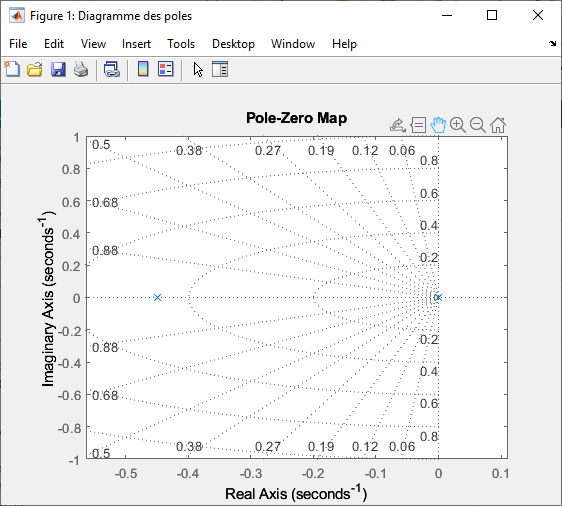
\includegraphics[width=0.5\linewidth]{pzmap112.PNG}
    \caption{Diagramme des pôles et des zéros du système H(s)}
    \label{fig:pzmap112}
\end{figure}
On remarque que notre système est critiquement stable, car on a un pôle $p_1=0$ de multiplicité 1 et un pôle à partie réelle nulle ($s=-5$).
\subsection{}
La réponse indicielle du système nous est donnée par
\begin{equation*}
    y_{ind}(t)=\Lp^{-1}[H(s)\frac{1}{s}](s)
\end{equation*}
On a d'après les théorèmes de la valeur initiale et de la valeur finale :
\begin{align*}
    y_{ind}(0^+)&=\lim_{|s|\rightarrow+\infty}sH(s)\frac{1}{s}=\lim_{|s|\rightarrow0}H(s)\\
    H(s)&=_{s\rightarrow+\infty}=\frac{b}{s^2+o(s^2)}\sim\frac{b}{s^2}\\
    H(s)&=\lim_{|s|\rightarrow+\infty}H(s)=0\\
    y_{ind}(+\infty)&=\lim_{|s|\rightarrow0}sH(s)\frac{1}{s}=\lim_{|s|\rightarrow0}H(s)\\
    H(s)&\sim_{s\rightarrow0}=\frac{b}{as)}\\
    H(s)&=\lim_{|s|\rightarrow+\infty}H(s)=+\infty\\
\end{align*}
Ce qui correspond au graphique obtenu figure \ref{fig:step113}
\begin{figure}[h]
    \centering
    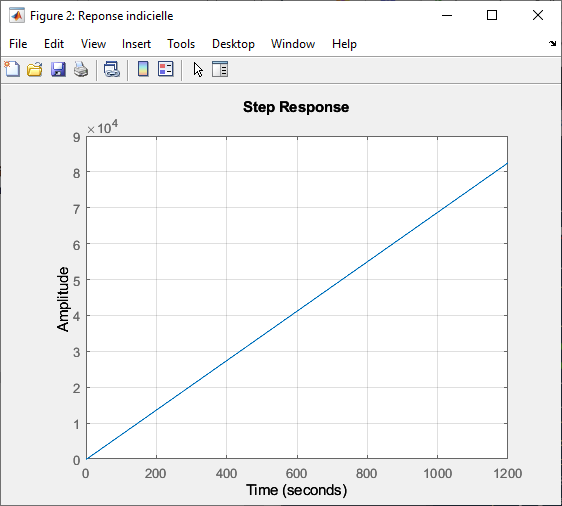
\includegraphics[width=0.5\linewidth]{step113.PNG}
    \caption{Réponse indicielle du système}
    \label{fig:step113}
\end{figure}
\subsection{}
On calcule les valeurs asymptotiques du lieu de Nyquist :
\begin{align*}
    H(j\omega)&=\frac{b}{(j\omega+a)j\omega}=\frac{b}{-\omega^2+ja\omega}=\frac{b}{-\omega^2+ja\omega}\frac{-\omega^2-ja\omega}{-\omega^2-ja\omega}\\
    &=\frac{-b\omega^2-jab\omega}{\omega^4+(a\omega)^2}=-\frac{b}{\omega^2+a^2}-j\frac{ab}{\omega^3+a^2\omega}\\
    H(j\omega)&\sim_{\omega\rightarrow0}-\frac{b}{a^2}-j\frac{b}{a\omega}\text{ donc }\begin{cases}
        Re(H(j\omega))=-\frac{b}{a^2}\approx-153\\
        Im(H(j\omega))=-\frac{b}{a\omega}\rightarrow+\infty
    \end{cases}\\
    H(j\omega)&\sim_{\omega\rightarrow+\infty}-\frac{b}{\omega^2}-j\frac{ab}{\omega^3}\text{ donc }\begin{cases}
        Re(H(j\omega))=-\frac{b}{\omega^2}\rightarrow0\\
        Im(H(j\omega))=-\frac{ab}{\omega^3}\rightarrow0
    \end{cases}\\
\end{align*}
Ces valeurs sont confirmées par le lieu obtenu figure \ref{fig:nyquist114}
\begin{figure}[h]
    \centering
    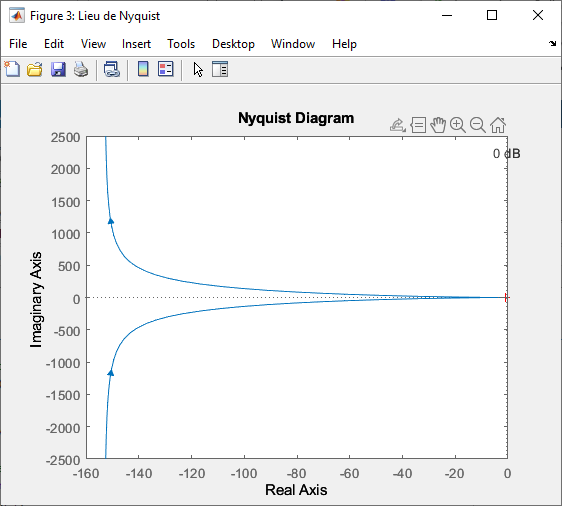
\includegraphics[width=0.5\linewidth]{nysquist114.PNG}
    \caption{Lieu de Nyquist du système}
    \label{fig:nyquist114}
\end{figure}
\subsection{}
On obtient le diagramme de Bode présenté dans la figure \ref{fig:bode115}.
On remarque dans un premier temps une pente de -20db/dec, et ceci depuis le début. Cette pente est induite par notre premier pôle en $\omega=0$. On remarque ensuite une pente à -40db/dec à partir de $\omega=0.45$ ce qui correspond à notre deuxième pôle. Le diagramme de Bode a pour valeur asymptotique $+\infty$ pour la marge en 0, $-\infty$ pour le gain en $+\infty$, $-\frac{\pi}{2}$ pour la phase en 0 et $-\pi$ pour la phase en $+\infty$.
\begin{figure}[h]
    \centering
    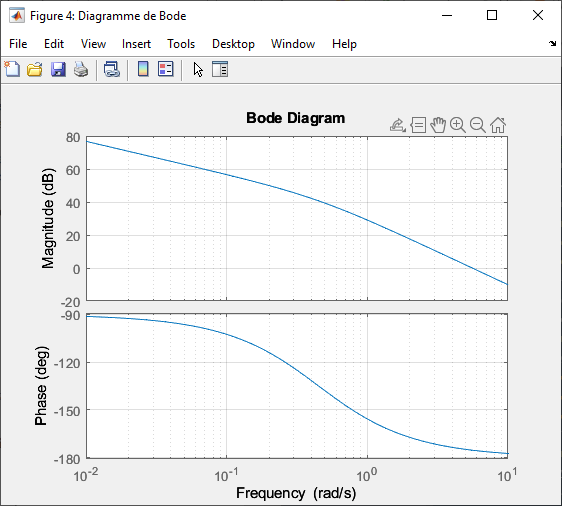
\includegraphics[width=0.5\linewidth]{bode115.PNG}
    \caption{Diagramme de Bode du système}
    \label{fig:bode115}
\end{figure}
\section{Commande Proportionnelle}
\subsection{}
\begin{align*}
    H_0(s)&=C_p(s)H(s)=\frac{N_0(s)}{D_0(s)}=\frac{K_Cb}{s(s+a)}\\
    H_f(s)&=\frac{N_0(s)}{N_0(s)+D_0(s)}=\frac{K_Cb}{K_Cb+s(s+a)}\\
    H_e(s)&=\frac{D_0(s)}{N_0(s)+D_0(s)}=\frac{s(s+a)}{K_Cb+s(s+a)}\\
    D_f(s)&=N_0(s)+D_0(s)=K_Cb+s(s+a)\\
\end{align*}
\subsection{}
L'erreur dynamique $e_1$ nous est donnée par :
\begin{equation*}
    e_1=\lim_{s\rightarrow0}H_e(s)\frac{1}{s}=\lim_{s\rightarrow0}\frac{s(s+a)}{K_Cb+s(s+a)}\frac{1}{s}=\lim_{s\rightarrow0}\frac{s+a}{K_cb+sa+s^2}=\frac{a}{K_cb}
\end{equation*}
On veut que l'erreur dynamique soit inférieure à 1\% soit :
\begin{equation*}
    e_1<1\%\Leftrightarrow\frac{a}{K_Cb}<1\%\Leftrightarrow K_C>\frac{a}{0.01b}\Leftrightarrow K_C>1.45
\end{equation*}
\subsection{}
On obtient le lieu des pôles figure \ref{fig:rlocus123}. On remarque que le système est toujours stable pour toutes les valeurs de $K_C>0$. Le système est critiquement stable pour $K_C=0$.
\begin{figure}[h]
    \centering
    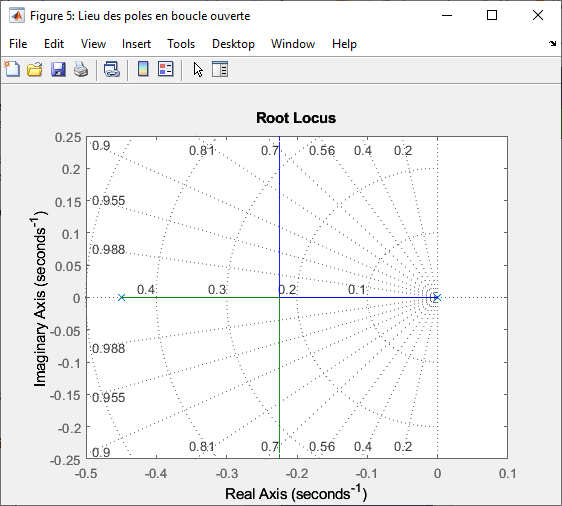
\includegraphics[width=0.5\linewidth]{rlocus123.PNG}
    \caption{Lieu des pôles du système avec correcteur proportionnel}
    \label{fig:rlocus123}
\end{figure}
\subsection{}
En étudiant le diagramme de Bode figure \ref{fig:bode124}, on observe une marge de phase initiale de 5°, pour obtenir une marge de phase supérieure a 45° il faut descendre la courbe de gain d'au minimum 40dB, soit :
$$
    20\log(K_C)<-40\Leftrightarrow K_C<10^{-2}\Leftrightarrow K_C<0.01
$$
\begin{figure}[h]
    \centering
    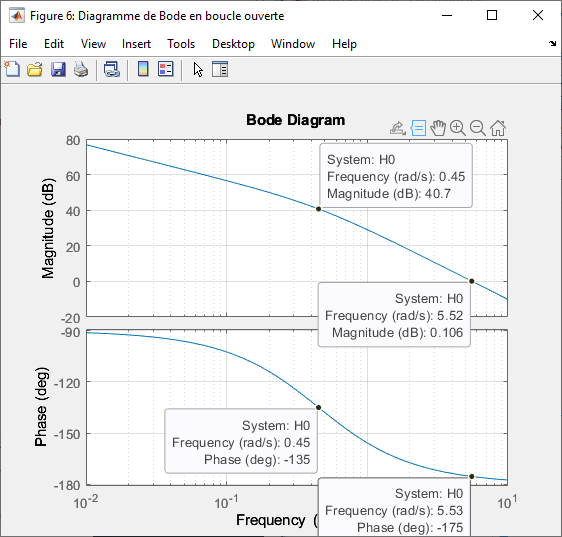
\includegraphics[width=0.5\linewidth]{bode124.PNG}
    \caption{Diagramme de Bode du système avec correcteur proportionnel de valeur 1}
    \label{fig:bode124}
\end{figure}

On peut remarquer les variations de gain et de phases induites par les pôles sur notre diagramme de Bode, les pôles induisant chacun une variation de la pente de -20db/dec.
\begin{figure}[h]
    \centering
    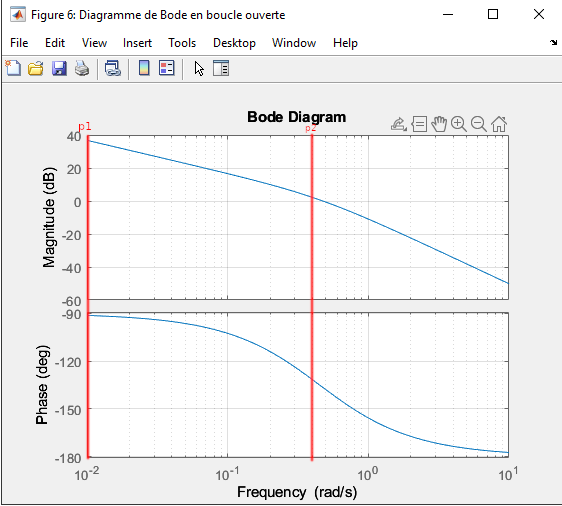
\includegraphics[width=0.5\linewidth]{bode124_2.PNG}
    \caption{Diagramme de Bode du système avec un correcteur proportionnel de valeur 0.01}
\end{figure}
\subsection{}
On a trouvé que pour satisfaire les conditions de précision, notre correcteur devait avoir une valeur supérieure à 1.45. Or, nous avons trouvé à la question précédente qu'il fallait une valeur de correcteur inférieure à 0.01 afin de respecter les conditions de stabilité. On en déduit alors qu'il est impossible de satisfaire les conditions de stabilité et de précision simultanément avec notre correcteur proportionnel.
\subsection{}
On choisit afin de satisfaire au mieux les deux conditions une valeur entre 0.01 et 1.45, ici, on prendra $K_C=0.1$, qui correspond à une erreur dynamique de 15\%.
On peut alors tracer le diagramme de Bode et relever une marge de phase de 5° et une marge de gain qui tend vers l'infini.

En observant la réponse indicielle, on peut relever que le temps de montée de 655 ms, un temps d'établissement de 13 secondes. On trouve également un dépassement ayant un temps de 1.81 seconde d'une valeur de 81\%.
\begin{figure}
    \centering
    \begin{subfigure}[b]{0.4\textwidth}
        \centering
        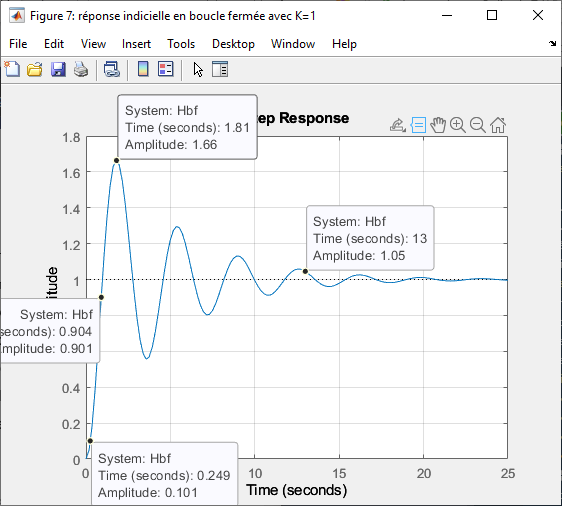
\includegraphics[width=\textwidth]{step126.PNG}
        \caption{Réponse indicielle}
        \label{fig:step126}
    \end{subfigure}
    \hfill
    \begin{subfigure}[b]{0.4\textwidth}
        \centering
        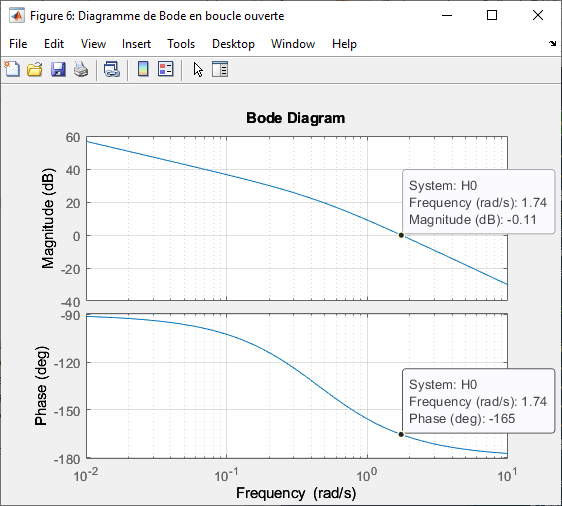
\includegraphics[width=\textwidth]{bode126.PNG}
        \caption{Diagramme de Bode}
        \label{fig:bode126}
    \end{subfigure}
    \caption{Diagrammes du système pour un correcteur proportionnel de 0.1}
\end{figure}
\section{Commande Proportionnelle Dérivée Filtrée}
\subsection{}
Le correcteur a pour expression
\begin{equation*}
    C_1(s)=K_C(1+\frac{T_Ds}{1+T_fs}
\end{equation*}
On cherche le pôle $p_c$ et le zéro $z_c$ du correcteur. Commençons par simplifier la fonction de transfert du correcteur en un quotient.
\begin{align*}
    C_1(s)&=K_C(\frac{1+T_fs}{1+T_fs}+\frac{T_Ds}{1+T_fs})\\
    &=K_C\frac{1+(T_f+T_D)s}{1+T_fs}=\frac{N_{C_1}(s)}{D_{C_1}(s)}\\
    &=K_C\frac{1+(1+\frac{1}{\alpha})T_Ds}{1+\frac{T_D}{\alpha}s}
\end{align*}
On peut désormais trouver les pôles et les zéros en résolvant les équations suivantes :
\begin{align*}
    N_{C_1}(z_c)&=0\\
    \Leftrightarrow K_C(1+(T_f+T_D)z_c)&=0\\
    \Leftrightarrow z_c=-\frac{1}{T_f+T_D}&=-\frac{1}{T_D(1+\frac{1}{\alpha})}\\
    D_{C_1}(p_c)&=0\\
    \Leftrightarrow 1+T_fp_c&=0\\
    \Leftrightarrow p_c&=-\frac{\alpha}{T_D}
\end{align*}
\subsection{}
\begin{align*}
    H(s)&=\frac{b}{s(s+a)}\\
    p_1&=0\\
    p_2&=-a\\
    C_1(s)H(s)&=K_C\frac{1+(1+\frac{1}{\alpha}T_Ds}{1+\frac{1}{\alpha}T_Ds}\frac{b}{s(s+a)}\\
    1+(1+\frac{1}{\alpha})T_Ds=s+a&\text{ ou }1+(1+\frac{1}{\alpha})T_Ds=1+\frac{1}{a}\\
    T_D&=\frac{\alpha}{\alpha+1}\frac{1}{a}
\end{align*}
On a alors $T_D=2.12$sec.
\subsection{}
On peut tracer le diagramme de bode du correcteur et relever le pole et le zéro comme sur la figure \ref{fig:bode133}
\begin{figure}[h]
    \centering
    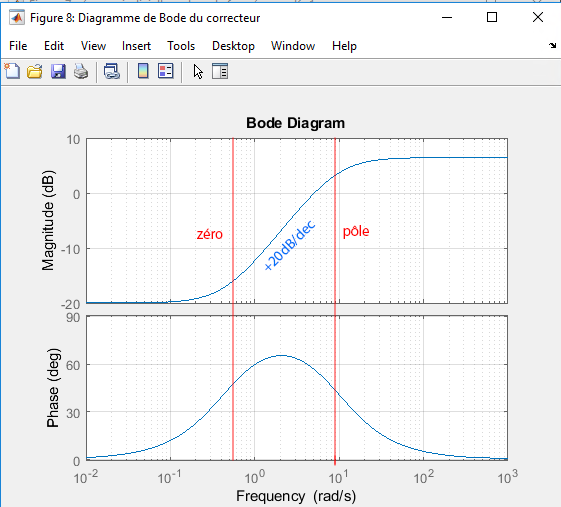
\includegraphics[width=0.5\linewidth]{bode133.png}
    \caption{Diagramme de Bode du correcteur $C_1$}
    \label{fig:bode133}
\end{figure}
\subsection{}
\begin{align*}
    H_{01}(s)&=C_1(s)H(s)=\frac{N_0(s)}{D_0(s)}=K_C\left(\frac{1+(1+\frac{1}{\alpha})T_Ds}{1+\frac{1}{\alpha}T_Ds}\right)\frac{b}{as(1+\frac{1}{\alpha}s}\\
    &=\frac{K_C\frac{b}{a}}{(1+\frac{1}{\alpha}T_Ds)s}\\
    H_{f1}(s)&=\frac{N_0(s)}{N_0(s)+D_0(s)}=\frac{K_C\frac{b}{a}}{K_C\frac{b}{a}+(1+\frac{1}{\alpha}T_Ds)s}\\
    H_{e1}(s)&=\frac{D_0(s)}{N_0(s)+D_0(s)}=\frac{(1+\frac{1}{\alpha}T_Ds)s}{K_C\frac{b}{a}+(1+\frac{1}{\alpha}T_Ds)s}\\
    D_{f1}(s)&=N_0(s)+D_0(s)=K_C\frac{b}{a}+(1+\frac{1}{\alpha}T_Ds)s\\
\end{align*}
\subsection{}
L'erreur statique est définie par 
\begin{equation*}
    e_0=\lim_{s\rightarrow0}H_{e1}(s)=0
\end{equation*}
Donc notre correcteur induit une erreur statique nulle.
\subsection{}
L'erreur dynamique est définie par 
\begin{equation*}
    e_1=\lim_{s\rightarrow0}H_{e1}(s)\frac{1}{s}=\frac{a}{K_{C1}b}
\end{equation*}
\subsection{}
On peut relever sur le diagramme de Bode (cf figure \ref{fig:bode137}) de notre fonction de transfert en boucle ouverte une marge de phase de 21° et une marge de gain infinie.
\begin{figure}[h]
    \centering
    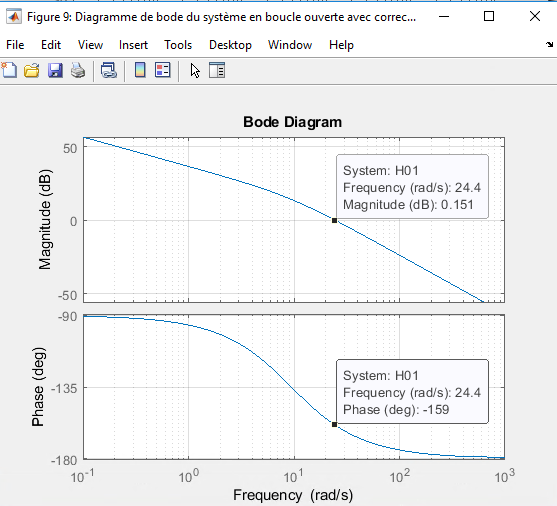
\includegraphics[width=0.5\linewidth]{bode137.png}
    \caption{Diagramme de bode de $H_{01}$}
    \label{fig:bode137}
\end{figure}
\subsection{}
On obtient les graphiques de la figure \ref{fig:sisotool128} en utilisant la fonction sisotool.
\begin{figure}[h]
    \centering
    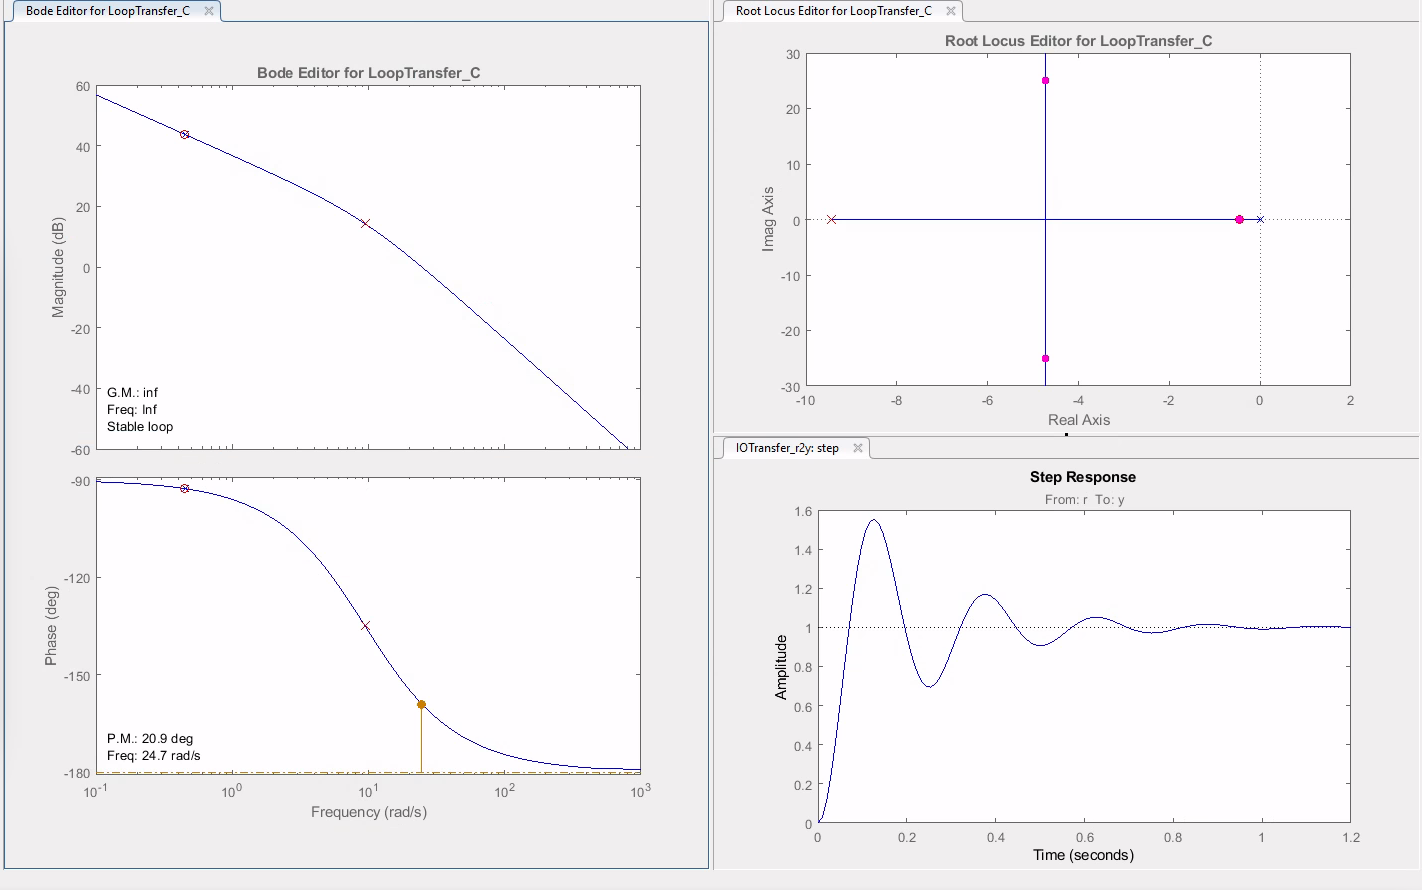
\includegraphics[width=1\linewidth]{sisotool138.png}
    \caption{Graphiques sur sisotool}
    \label{fig:sisotool128}
\end{figure}
\subsection{}
On remarque sur le lieu des poles de la figure \ref{fig:sisotool128} que le pôle situé en $\approx-9.43$ se déplace vers 0 quand le gain augmente.
\subsection{}
En augmentant le gain $K_{C1}$, on remarque que les oscillations augmente, on a donc $\xi$ qui diminue et tend vers 0 donc le système admet une résonance car $\xi<0.7$. En revanche, si on diminue le gain $K_{C1}$ entre 1 et 0, on remarque que $\xi$ augmente et la résonance disparait, le système est amorti.
\subsection{}
On trouve que pour une valeur de $K_{C1}=0.19$, on a une marge de phase qui vaut $\approx45$°. Les pôles se trouvent dans le demi-plan gauche du lieu des pôles, on a donc une stabilité en cette valeur.
L'erreur dynamique est donc de $e_1=\frac{a}{K_{C1}b}\approx8\%$.
\begin{figure}
    \centering
    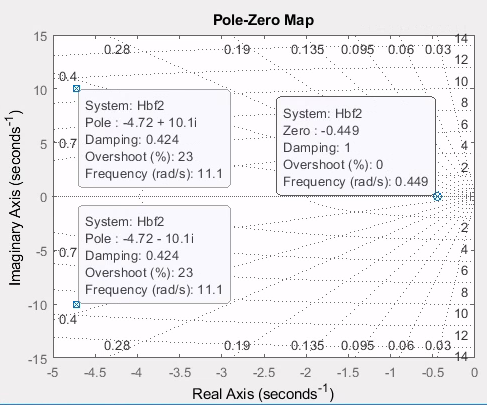
\includegraphics[width=0.75\linewidth]{pzmap1311.png}
    \caption{Diagramme des pôles}
    \label{fig:pzmap1311}
\end{figure}
On remarque 3 poles:
\begin{itemize}
    \item Un premier pôle, lié à un zéro, de module 0.449 et de coefficient d'amortissement de 1 (ce pôle n'influe pas sur les oscillations du système).
    \item Deux pôles complexes conjugués, de module 11.15 et de coefficient d'amortissement de 0.424 (ces pôles vont donc provoquer une oscillation).
\end{itemize}
\end{document}
